% TÉCNICAS E FERRAMENTAS ------------------------------------------------------------------

\chapter{PROPOSTA}
\label{chap:proposta}

Neste capítulo serão expostas as tecnologias e ferramentas que serão utilizadas no desenvolvimento do aplicativo, bem como a metodologia que será seguida para o gerenciamento de tarefas.

\section{TECNOLOGIAS}
\label{sec:tecnologias}

A presente proposta diz respeito ao desenvolvimento de um sistema \textit{web}. Um sistema \textit{web} consiste em um programa de computador instalado em um servidor HTTP, que disponibiliza páginas \textit{web} para os clientes HTTP como \textit{web browsers}.

As tecnologias necessárias para o desenvolvimento da aplicação identificadas serão descritas abaixo.

\subsection{Unified Modeling Language}
\label{sub:uml}

A UML foi adotada como a linguagem de modelagem de sistema, pois com ela conseguimos facilmente representar comportamentos e necessidades do sistema em nível de software e \textit{hardware}. Os diagramas a serem modelados e suas respectivas funções são:

\begin{itemize}
    \item \textbf{Diagrama de Caso de Uso}, que fornecerá uma visão geral das funcionalidades do aplicativo.
    
    \item \textbf{Diagrama de Classe}, que possibilita o desenvolvedor entender a organização das classes e seus relacionamentos.
    
    \item \textbf{Diagrama de Implantação}, que proporciona uma visão de alto nível acerca das necessidade de hardware e software para a implantação da aplicação.
    
    \item \textbf{Diagrama Entidade-Relacionamento}, permite entender a organização dos dados nas tabelas, bem como os atributos, relacionamentos e restrições.
\end{itemize}

\subsection{MySQL}
\label{sub:rdb}

O MySQL será o SGBD para a persistência de dados. Ele foi escolhido devido à sua confiabilidade, consistência e normalização ante aos modelo não relacionais. É um sistema gratuito, amplamente utilizado em aplicações de todos os tamanhos. O uso desse SGBD utilizado pelo aplicativo da Uber \cite{klitzkeevan2016} e no portal openNASA \cite{howardalex2011}.

A modelagem do banco de dados foi feita utilizando a ferramenta MySQL Workbench e pode ser visualizado na \autoref{fig:diagramaer}. Já o dicionário de dados está disponível na \autoref{sec:titSecDiagERDicionario}.

\subsection{PHP}
\label{sub:php}

O Pre-hypertext Processor (PHP) é uma linguagem interpretada criada em 1995 por Rasmus Lerdorf. Amplamente utilizada no desenvolvimento de aplicações web, a linguagem evoluiu e passou a oferecer funcionalidades na linha de comando. Ela está presente no código fonte de grandes aplicações como Magento, WordPress, Drupal, Wikipédia e Facebook (até 2018) \cite{emmottfred2019}.

No presente projeto esta linguagem será utilizada no backend, por meio do Laravel Framework.

\subsection{Laravel \textit{Framework}}
\label{sub:laravel}

\citeonline{Sommerville10} afirma que, “os frameworks dão suporte ao reúso de projeto, bem como ao reúso de classes específicas de sistema, pois fornecem uma arquitetura de esqueleto para a aplicação”.

De acordo com \citeonline{otwelltaylor2019}, o Laravel é "um framework de aplicação web com sintaxe expressiva e elegante". Sua primeira versão foi lançada no dia em 9 de junho de 2011. No momento se encontra na versão 5.8, lançada em 26 de fevereiro de 2019.

Este é usado para a construção de grandes aplicações \textit{web} que utilizam o padrão arquitetural MVC, fornecendo ao desenvolvedor funcionalidades comuns às aplicações como roteamento e autenticação. Além de possuir uma poderosa Command-line Interface (CLI) chamado Artisan, que proporciona ao desenvolvedor facilidades para o desenvolvimento, como a criação de artefatos de código informando poucos parâmetros. Por exemplo, caso o desenvolvedor precise criar um recurso RESTful para cadastro de pessoas, ele pode facilitar o trabalho de criação dos arquivos de acordo com a \autoref{fig:artisanModel}.

\begin{figure}[H]
    \centering
    \caption{Exemplo do Artisan para a criação de \textit{model}, \textit{controller} e \textit{migration}}
    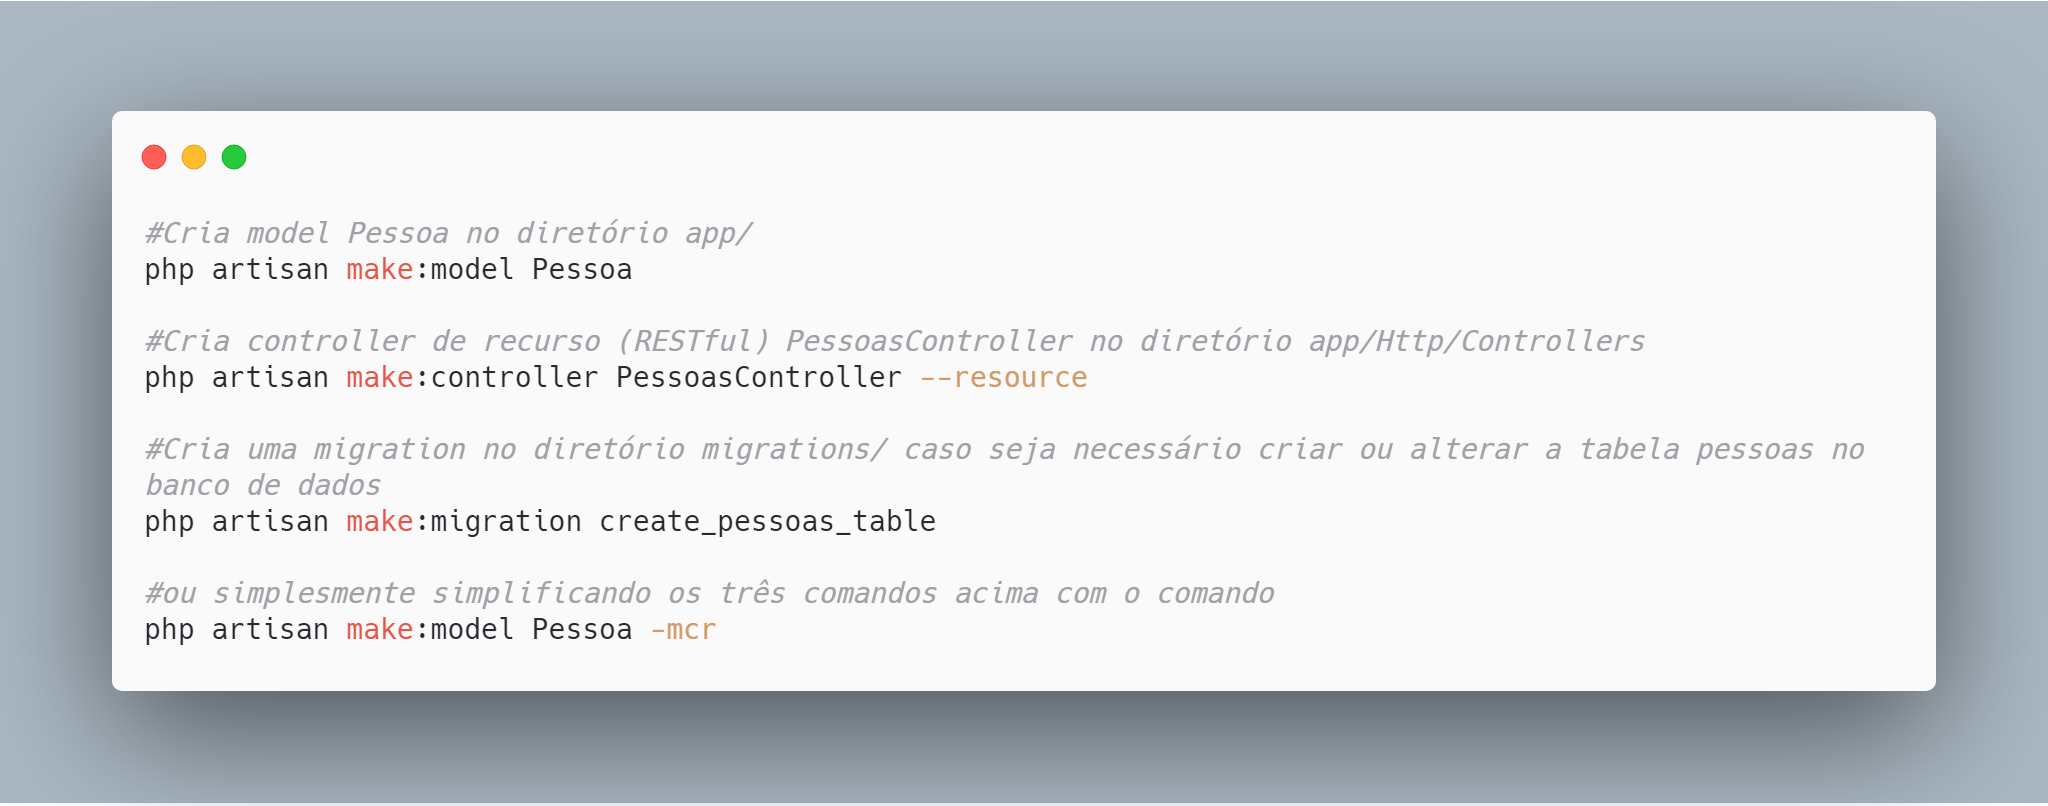
\includegraphics[width=13cm]{dados/figuras/php_artisan_make_model.png}
    \label{fig:artisanModel}
    \fonte{Autoria própria}
\end{figure}

O código fonte deste \textit{framework} se encontra no GitHub e possui cerca de 52.500 \textit{stars} ou \textit{likes}, e aproximadamente 500 contribuidores, sendo o framework backend, independente da linguagem, mais aclamado pelos desenvolvedores no mundo.

Algumas de suas principais características são a simplicidade da documentação e do motor de roteamento, o poderoso \textit{container} de injeção de dependências, suporte a múltiplos SGBD para armazenamento de sessões e \textit{cache}, um ORM intuitivo e expressivo, agnosticismo quanto SGBD para as migrações do sistema, o robusto suporte a tarefas agendadas em \textit{background} e transmissão de eventos em \textit{broadcast}.

\subsection{MVC com o Laravel}
\label{sub:mvclaravel}

A camada de \textit{model} do MVC é implementada no Laravel por meio do Eloquent ORM, que é uma implementação simples e amigável do padrão Active Record. Na \autoref{fig:modelEloquent} podemos observar as facilidades que este Object-Relational Mapper (ORM) traz para a manipulação de dados. Por padrão, os \textit{models} em uma aplicação desenvolvida com o Laravel se encontram no diretório \textit{app}.

\begin{figure}[H]
    \centering
    \caption{Exemplo de operações de busca usando o Eloquent ORM}
    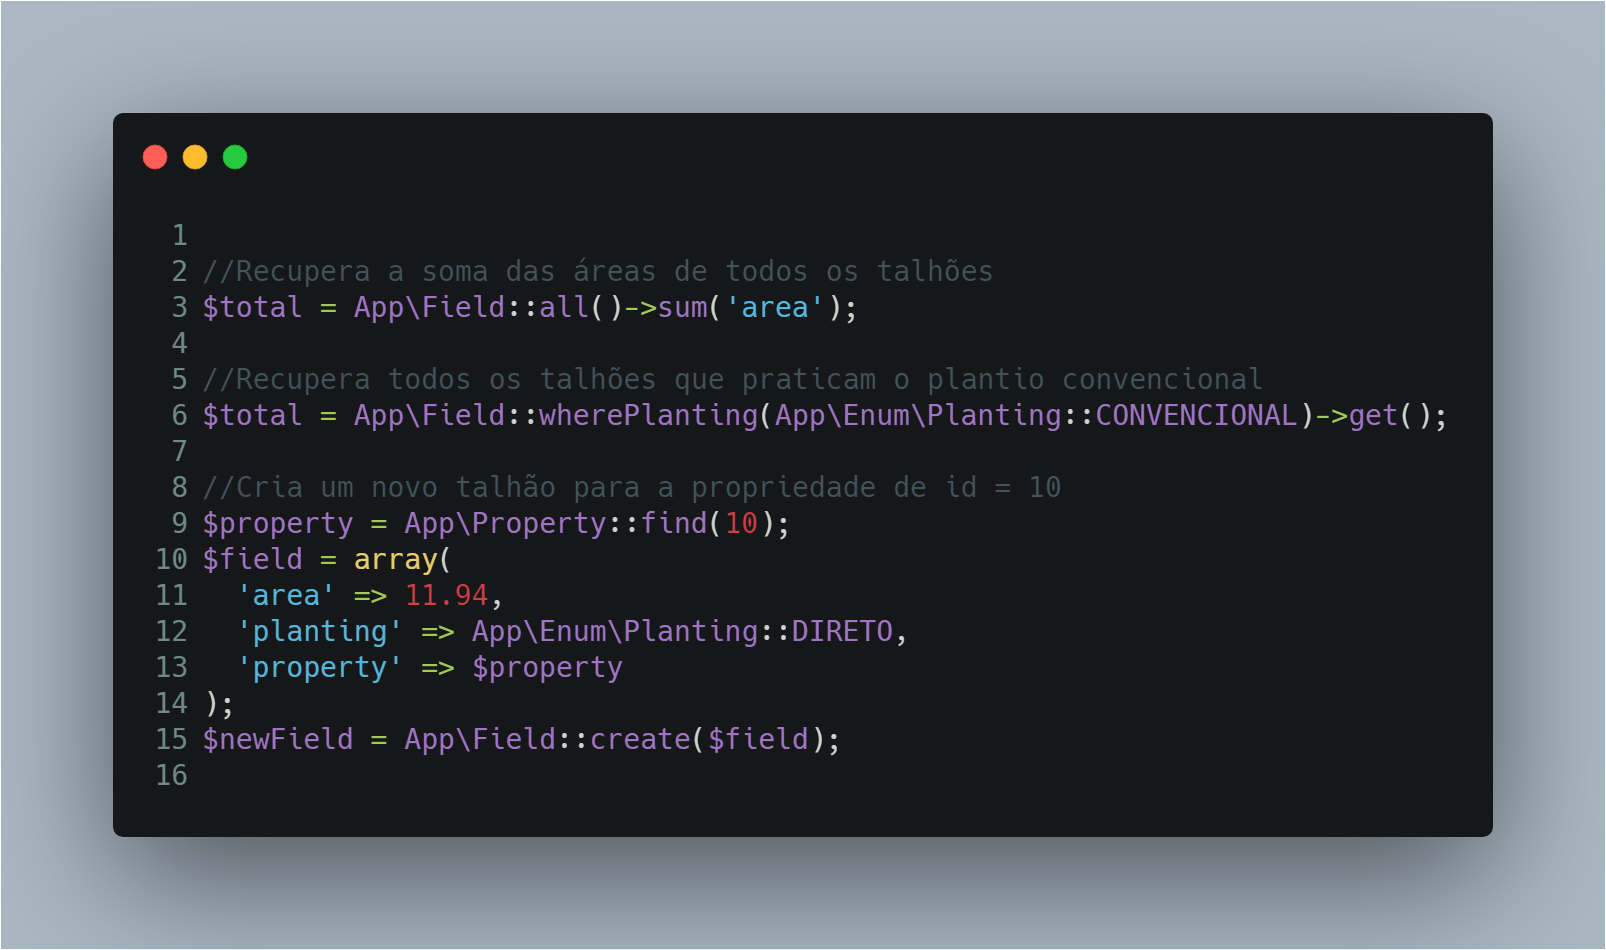
\includegraphics[width=13cm]{dados/figuras/exemplo_Model_Eloquent.png}
    \label{fig:modelEloquent}
    \fonte{Autoria própria}
\end{figure}

Na \autoref{fig:exemploRotas} é possível observar um exemplo de roteador utilizado no Laravel. O roteador é usado para determinar como será tratada uma requisição, dependendo de sua URI e verbo HTTP. No exemplo da \autoref{fig:exemploRotas}, é possível identificar quatro rotas possíveis no sistema. As chamadas são feitas usando a classe \textit{Route}, seguido de um método estático que representa o verbo HTTP da requisição, que recebe como o primeiro parâmetro a URI e no segundo o \textit{controller} seguido de um arroba e o nome do método que deverá tratar aquela requisição.

\begin{figure}[H]
    \centering
    \caption{Exemplo de roteador no Laravel}
    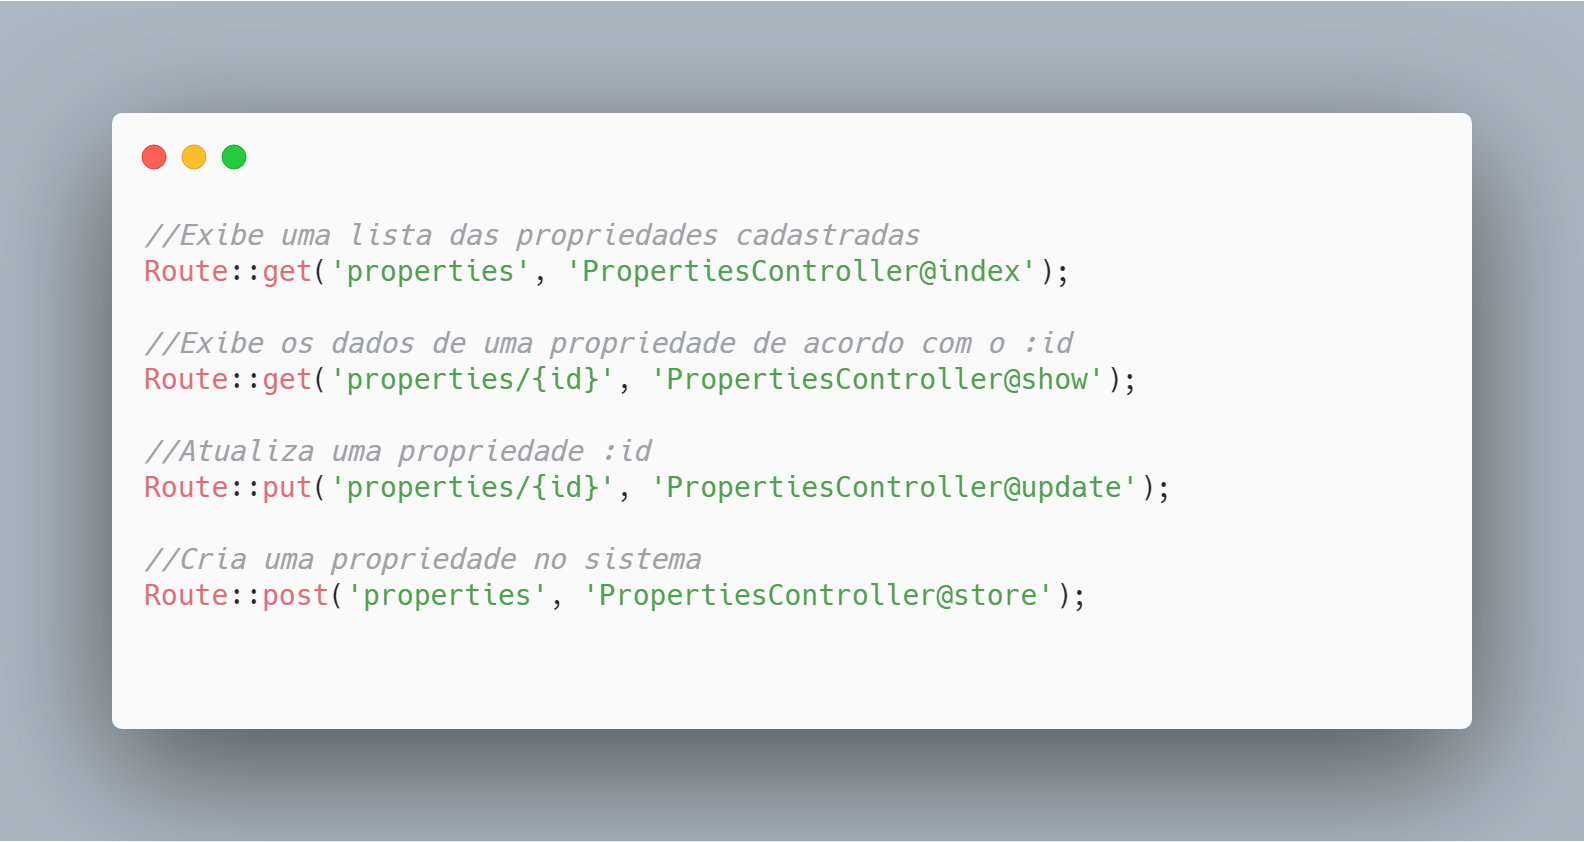
\includegraphics[width=13cm]{dados/figuras/exemplo_Rotas_Laravel.png}
    \label{fig:exemploRotas}
    \fonte{Autoria própria}
\end{figure}


No Laravel, por padrão, as classes \textit{controllers} se encontram no diretório App/Http/Controllers. Uma classe \textit{controller} no no Laravel não pode ser acessada diretamente, devendo o desenvolvedor criar rotas para este fim.

Na \autoref{fig:exemploController} é possível observar um exemplo de \textit{controller} no Laravel. O método \emph{store} é chamado quando uma requisição \emph{POST} é feita para a URI \emph{/properties}. Ao receber a requisição primeiramente é feita a validação dos dados e depois a criação do recurso na base de dados e então o usuário é redirecionada à listagem de propriedades.

\begin{figure}[H]
    \centering
    \caption{Exemplo de controller no Laravel}
    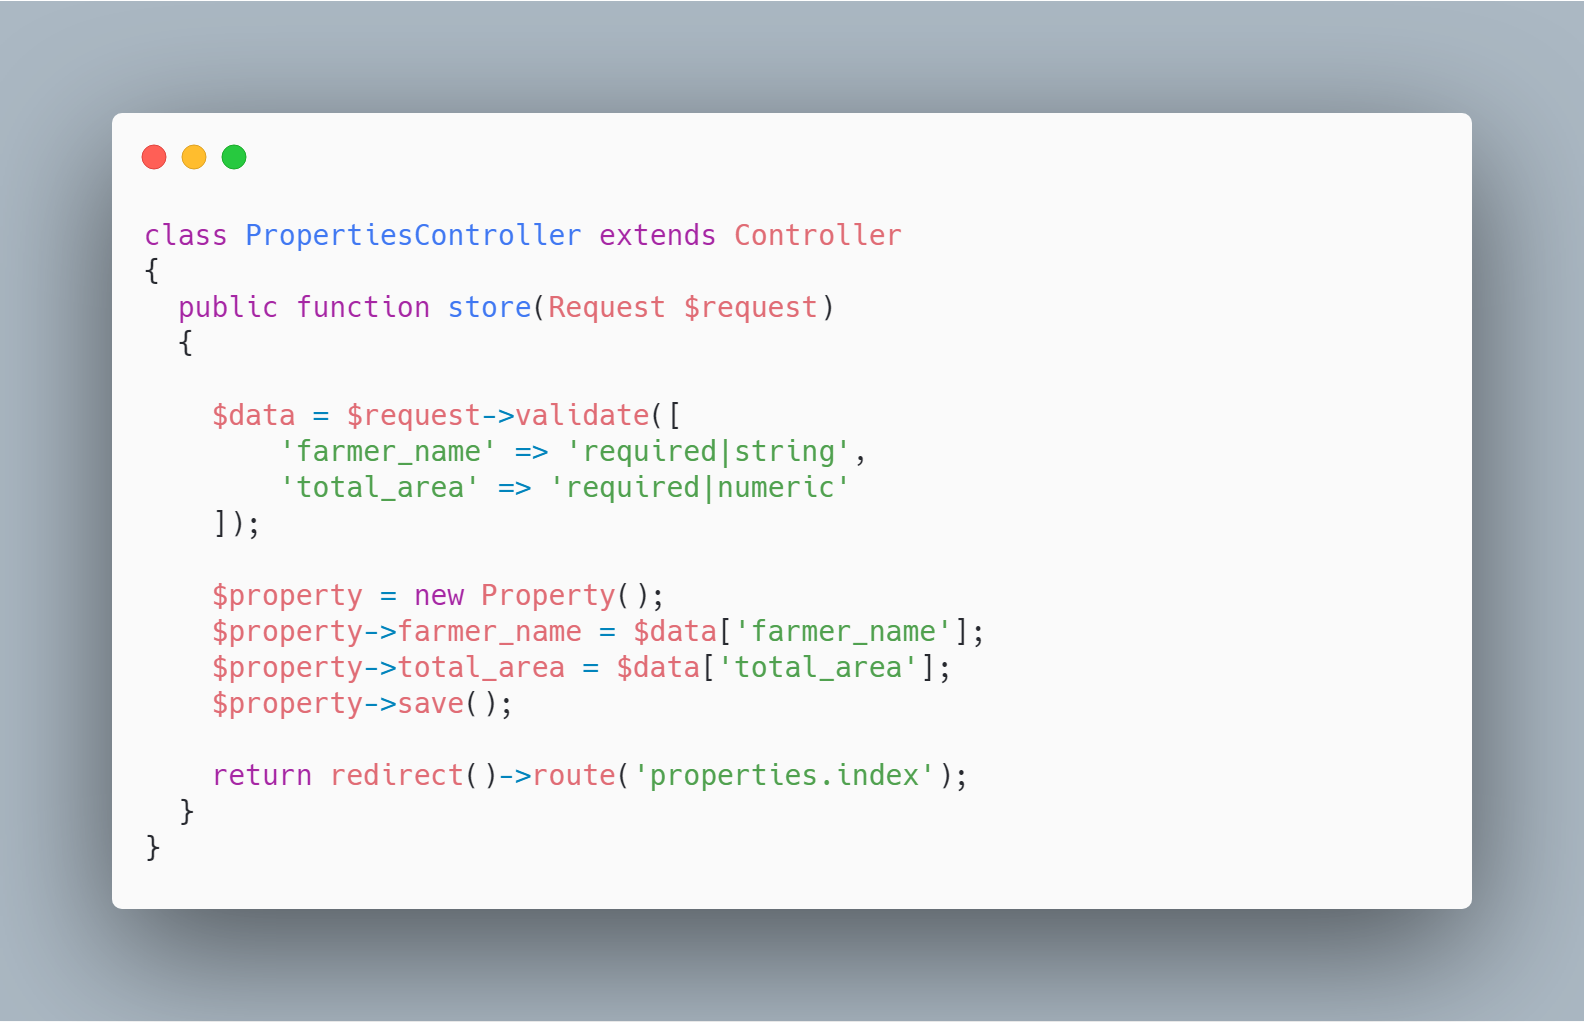
\includegraphics[width=13cm]{dados/figuras/exemplo_Controller_Laravel.png}
    \label{fig:exemploController}
    \fonte{Autoria própria}
\end{figure}

No desenvolvimento da presente aplicação a camada de \textit{view} não será implementada com o Laravel, sendo então repassada a responsabilidade de renderizar as informações no navegador para o React, descrito na \autoref{sub:react}.

\subsection{React}
\label{sub:react}

É uma biblioteca JavaScript mantida pela Facebook Inc. destinada principalmente à grandes aplicações, como o Facebook e Instagram, que devem atualizar uma grande quantidade de informações na tela em poucos segundos.

Essa biblioteca foi escolhida devido a característica da aplicação que deverá reagir aos inputs do usuário no formulário, informando os percentuais ideais de cada indicador químico na CTC, por exemplo. Além disso, possui uma documentação de fácil compreensão e uma das maiores comunidades, com milhares de perguntas e respostas para as mais diversas situações no StackOverflow e um repositório no GitHub com aproximadamente 130 mil \textit{stars} e 1300 contribuidores. 

A \autoref{fig:exemploViewReact} demonstra um exemplo de um componente do React. 

\begin{figure}[H]
    \centering
    \caption{Exemplo de componente com React}
    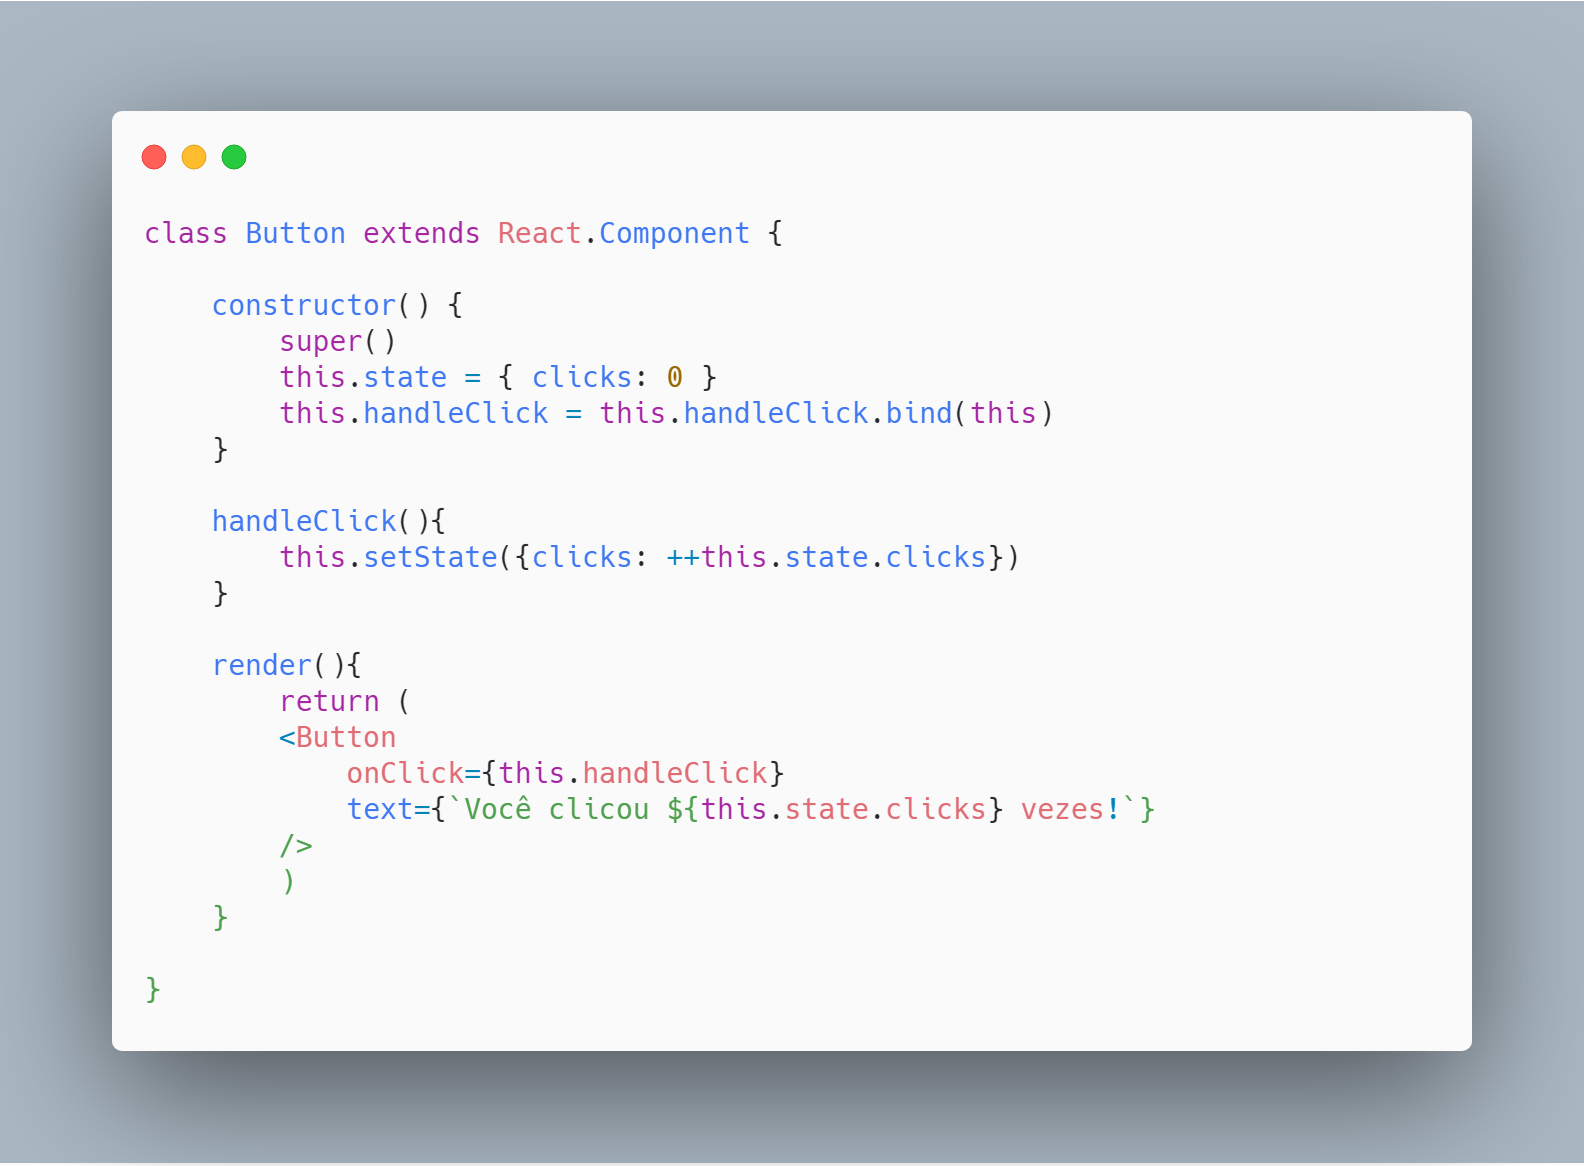
\includegraphics[width=13cm]{dados/figuras/exemplo_react_component.png}
    \label{fig:exemploViewReact}
    \fonte{Autoria própria}
\end{figure}

A \autoref{fig:exemploViewReact} apresenta o código JavaScript de um componente Button usando React. Esse código renderiza um botão que exibe um texto informando o usuário de quantas vezes aquele elemento foi clicado.

\subsection{Ant Design of React}
\label{sub:ant}

O Ant Design for React é uma biblioteca de componentes de interface para o React que pode ser requerida ao projeto por meio de um gerenciador de dependências como o Node Package Manager ou o Yarn. Ela fornece um conjunto de componentes de alta qualidade para o desenvolvimento de aplicações \textit{web}.

\subsection{Codeception}
\label{sub:codeception}

Para a escritas de teste de integração e unitários será utilizado o Codeception, um \textit{framework} para testes escrito em PHP que tem como objetivo facilitar a automação de testes em todas as camadas de um software.

Na \autoref{fig:excodeception} pode ser observado a facilidade de leitura e escrita de um teste de inusando Codeception.

\begin{figure}[H]
    \centering
    \caption{Exemplo de teste escrito com o Codeception}
    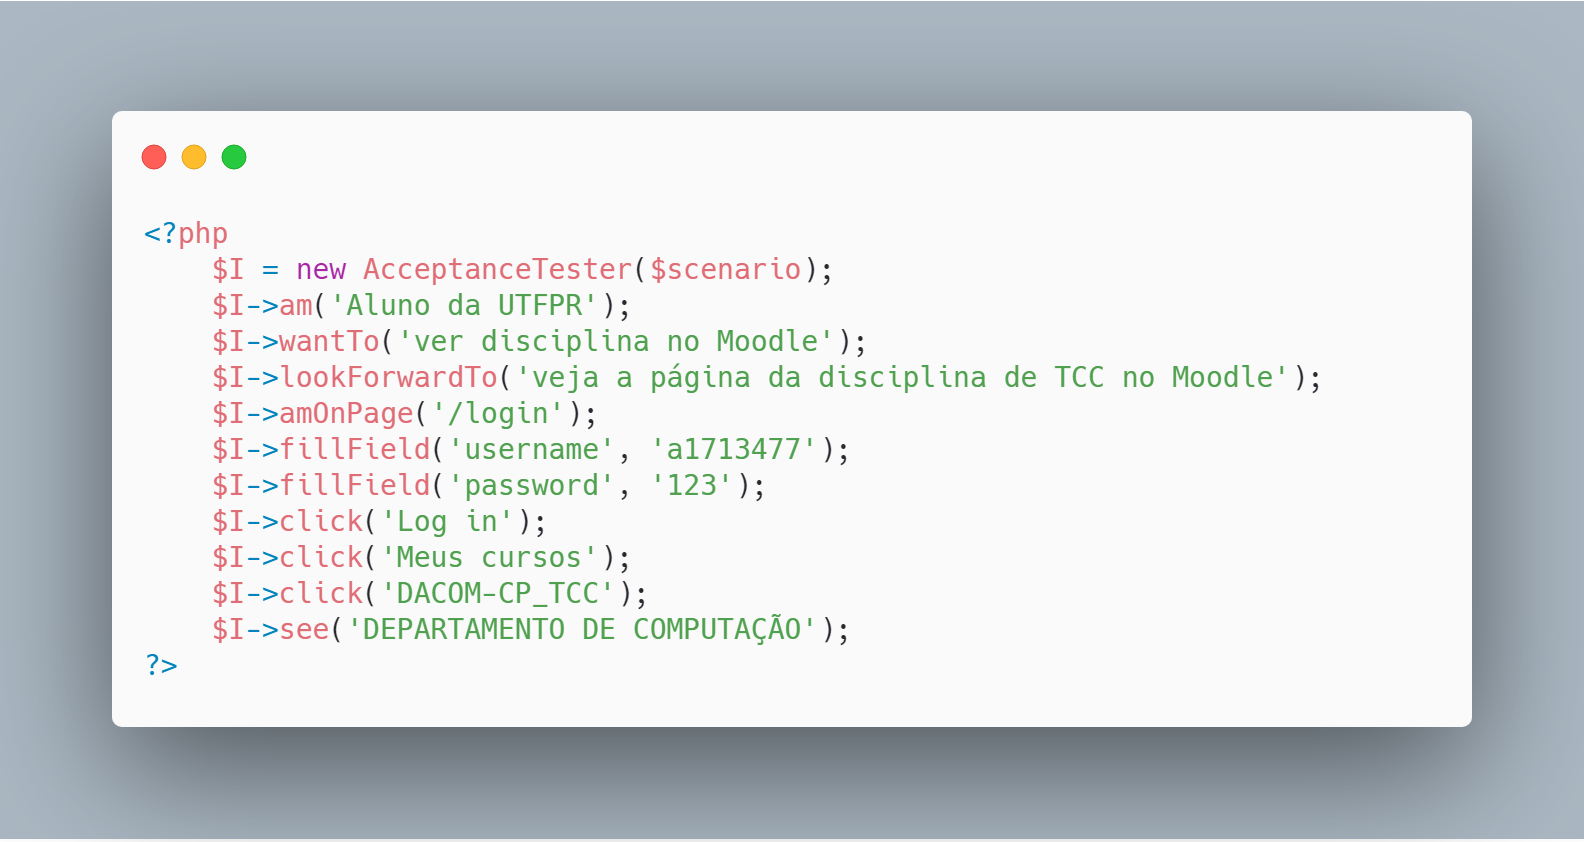
\includegraphics[width=13cm]{dados/figuras/teste_codeception.png}
    \label{fig:excodeception}
    \fonte{Autoria própria}
\end{figure}

\section{FERRAMENTAS}
\label{sec:ferramentas}
Nesta sessão serão apresentadas as ferramentas que serão úteis para o desenvolvimento e gerenciamento do projeto.

\subsection{Astah Community}
\label{sub:astah}

A ferramenta Astah Community é uma excelente ferramenta para modelagem UML. Por ser uma versão gratuita, possui algumas limitações. Apesar disso, essa versão satisfaz às necessidades do projeto visto que oferece suporte para a criação dos diagramas de caso de uso, classe e implantação.

\subsection{Trello}
\label{sub:trello}

O Trello é uma ferramenta de gerenciamento de projetos, simples e intuitiva baseada no conceito de kanban, recomendada para o gerenciamento de tarefas tanto individual quanto de equipes \cite{cardosopedro2016}.

Os projetos no Trello são representados por quadros. Dentro de cada quadro temos as listas, que aglomeram cartões. A menor configuração de listas recomendada em um projeto são em três listas: A fazer, fazendo e feito. Cada cartão representa uma tarefa e pode ser movido de uma lista para outra de acordo com o estado da tarefa.

Os cartões possuem diversas características, dentre as quais se destacam o prazo para conclusão, o rótulo, a possibilidade de criar \textit{checklists}, anexos e comentários.

\subsection{MySQL Workbench}
\label{sub:workbench}

O MySQL Workbench é uma ferramenta gratuita para a modelagem de dados, que auxilia os desenvolvedores na criação de modelos e administração de banco de dados MySQL. Ela possui diversas características muito úteis como a engenharia reversa e sincronização entre bases de dados.

Além disso, o Workbench é multiplataforma, oferecendo a aplicação nos ambientes Widnows, Linux e Mac OS. Ela fornece aos usuários diversas ferramentas para modelagem de banco de dados, realização de consultas com SQL e administração de banco.

\subsection{Visual Studio Code}
\label{sub:vscode}

O Visual Studio Code é uma ferramenta gratuita, de código aberto, que tem ganhado grande importância no cenário de desenvolvimento de software. Ela possui suporte a diversas linguagens de programação, dentre as quais o PHP e JavaScript, que serão as linguagens essenciais para a construção da aplicação.

\subsection{Git}
\label{sub:git}

A aplicação será versionada por meio do Git e terá o código-fonte hospedado no GitHub. O Git é um sistema de controle de versão de arquivos. Com ele é possível desenvolver projetos distribuídos de forma que toda alteração no código fonte é acompanhada. Com isso, vários desenvolvedores podem trabalhar no mesmo projeto sem risco de alterações. Sem o controle de versão, o desenvolvimento de aplicações se torna caótico.

\begin{figure}[H]
    \centering
    \caption{Demonstração do comportamento das \textit{branchs} no repositório Git}
    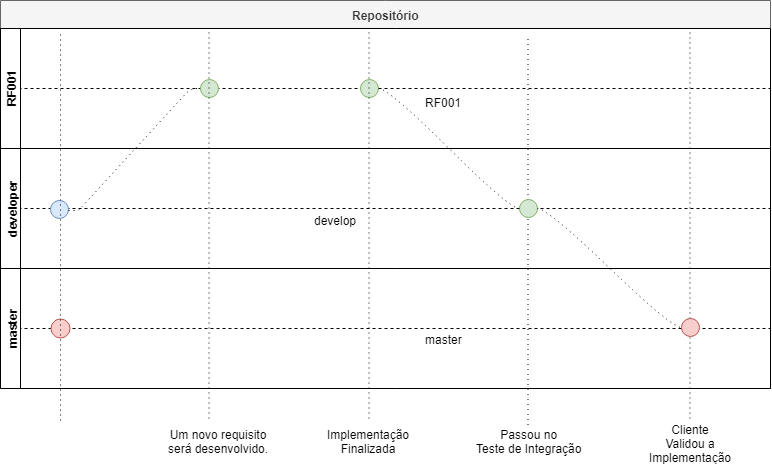
\includegraphics[width=13cm]{dados/figuras/git.png}
    \label{fig:exemplogit}
    \fonte{Autoria própria}
\end{figure}

Conforme exemplificado na \autoref{fig:exemplogit}, o repositório será divido em duas \textit{branches} principais: \textit{developer} e \textit{master}. A \textit{master} será a versão utilizada para a aplicação em produção. Enquanto a \textit{developer}, para o ambiente de homologação.

Quando uma nova funcionalidade precisa ser desenvolvida, é criada uma \textit{branch} específica a partir da versão de homologação. Após a conclusão da tarefa o desenvolvedor deve fazer um \textit{pull request} ou \textit{merge request} para a versão de homologação.

Caso tenha passado pelos testes e aprovada pelo cliente, então essa nova versão de homologação deverá ser unida com a master, gerando assim uma nova versão da aplicação. Após isso, o desenvolvedor deverá executar o \textit{pull} no servidor para versão de produção seja atualizada.

\section{METODOLOGIA}
\label{sec:metodologiadev}

Neste capítulo será apresentada a metodologia para o desenvolvimento da aplicação. Como o desenvolvimento da aplicação será realizado apenas por um desenvolvedor, fica inviável seguir um processo de software. Com isso, foi necessário uma adaptação de um modelo existente para o presente projeto. O modelo desenvolvido segue alguns traços do modelo iterativo-incremental, pois dos modelos consolidados disponíveis é o que mais se adéqua às mudanças no projeto, além de ser o modelo adotado pelo Scrum que influenciou a modelagem deste processo.

\subsection{Processo}
\label{sub:processo}
Nesta seção será explicada a \autoref{fig:modeloprocesso}, o fluxo dos requisitos do sistema desde a fase de análise até chegar na etapa de implementação.

\begin{figure}[H]
    \centering
    \caption{Modelo de aplicação do TDD no projeto}
    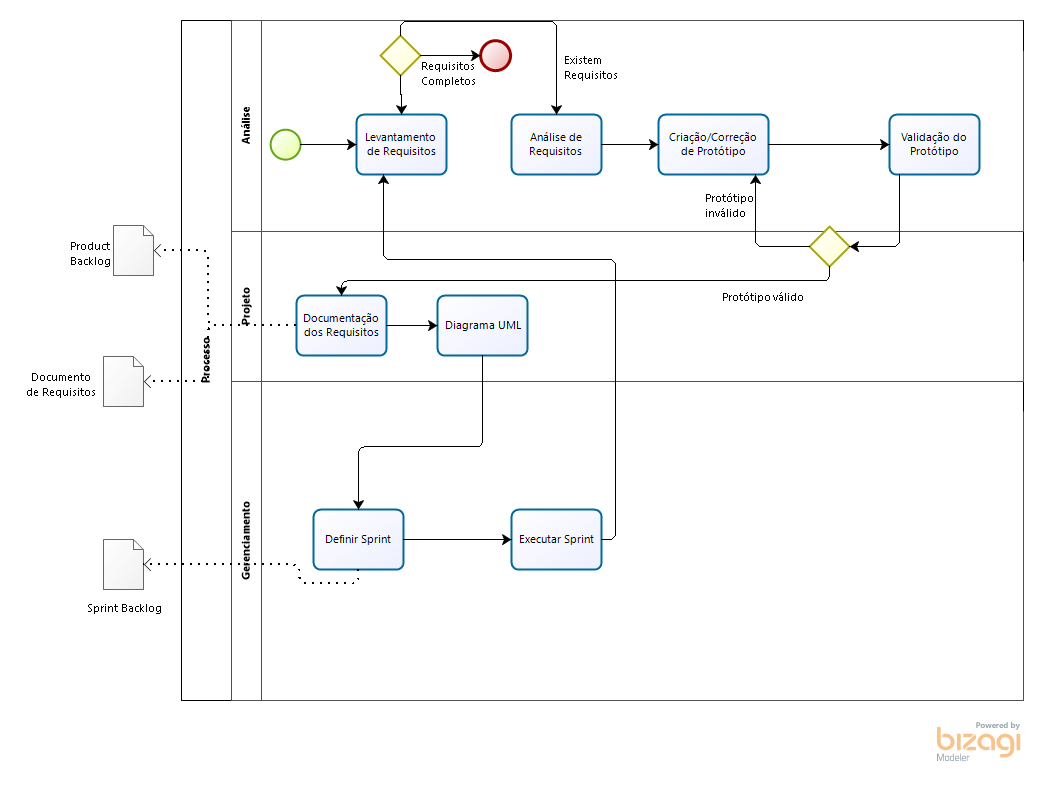
\includegraphics[width=13cm]{dados/figuras/ModeloDoProcesso.png}
    \label{fig:modeloprocesso}
    \fonte{Autoria própria}
\end{figure}

Primeiramente, é necessário o levantamento do requisitos, que é a etapa na qual o desenvolvedor deve entender qual é a necessidade do cliente. Existem diversos métodos para este fim, porém no presente projeto foi utilizado análise de documentos, no caso da planilha usado nos cálculos. Análise de requisitos foi feita em conjunto com o orientador, pois representa o cliente no projeto assim como o desenvolvimento dos protótipos. 

Após a análise foi iniciada a fase de projeto, Com os protótipos construídos, é dado início a etapa de documentação dos requisitos funcionais e não funcionais, além da especificação. Logo após, os diagramas da UML foram desenvolvidos, servindo de subsídios para a próxima fase.

Já na fase de gerenciamento são definidas as \textit{sprints}, formando o \textit{Sprint backlog} da próxima iteração da fase de implementação, descrita na \autoref{subsec:tdd}, que tem como entrada este artefato.

\subsection{Kanban}
\label{subsec:kanban}

Para o gerenciamento de tarefas, será utilizado o conceito de quadros \textit{kanban}, utilizando a ferramenta Trello. As tarefas serão divididas em seis quadros, demonstrados na \autoref{fig:trelloquadro}, que são:

\begin{itemize}
    \item \textbf{\textit{Product backlog}}: Os requisitos que foram definidos para o produto
    \item \textbf{\textit{Sprint backlog}}: Os requisitos que devem ser desenvolvidos na \textit{sprint} atual
    \item \textbf{\textit{Doing}}: Os requisitos que estão sendo desenvolvidos no momento
    \item \textbf{\textit{Done}}: Os requisitos que foram finalizados
    \item \textbf{\textit{Test}}: Os requisitos que após a finalização, foram enviados para teste em um servidor de homologação.
    \item \textbf{\textit{Deploy}}: Os requisitos que foram homologados e podem ir para produção.
\end{itemize}

\begin{figure}[H]
    \centering
    \caption{Quadro \textit{kanban} do projeto}
    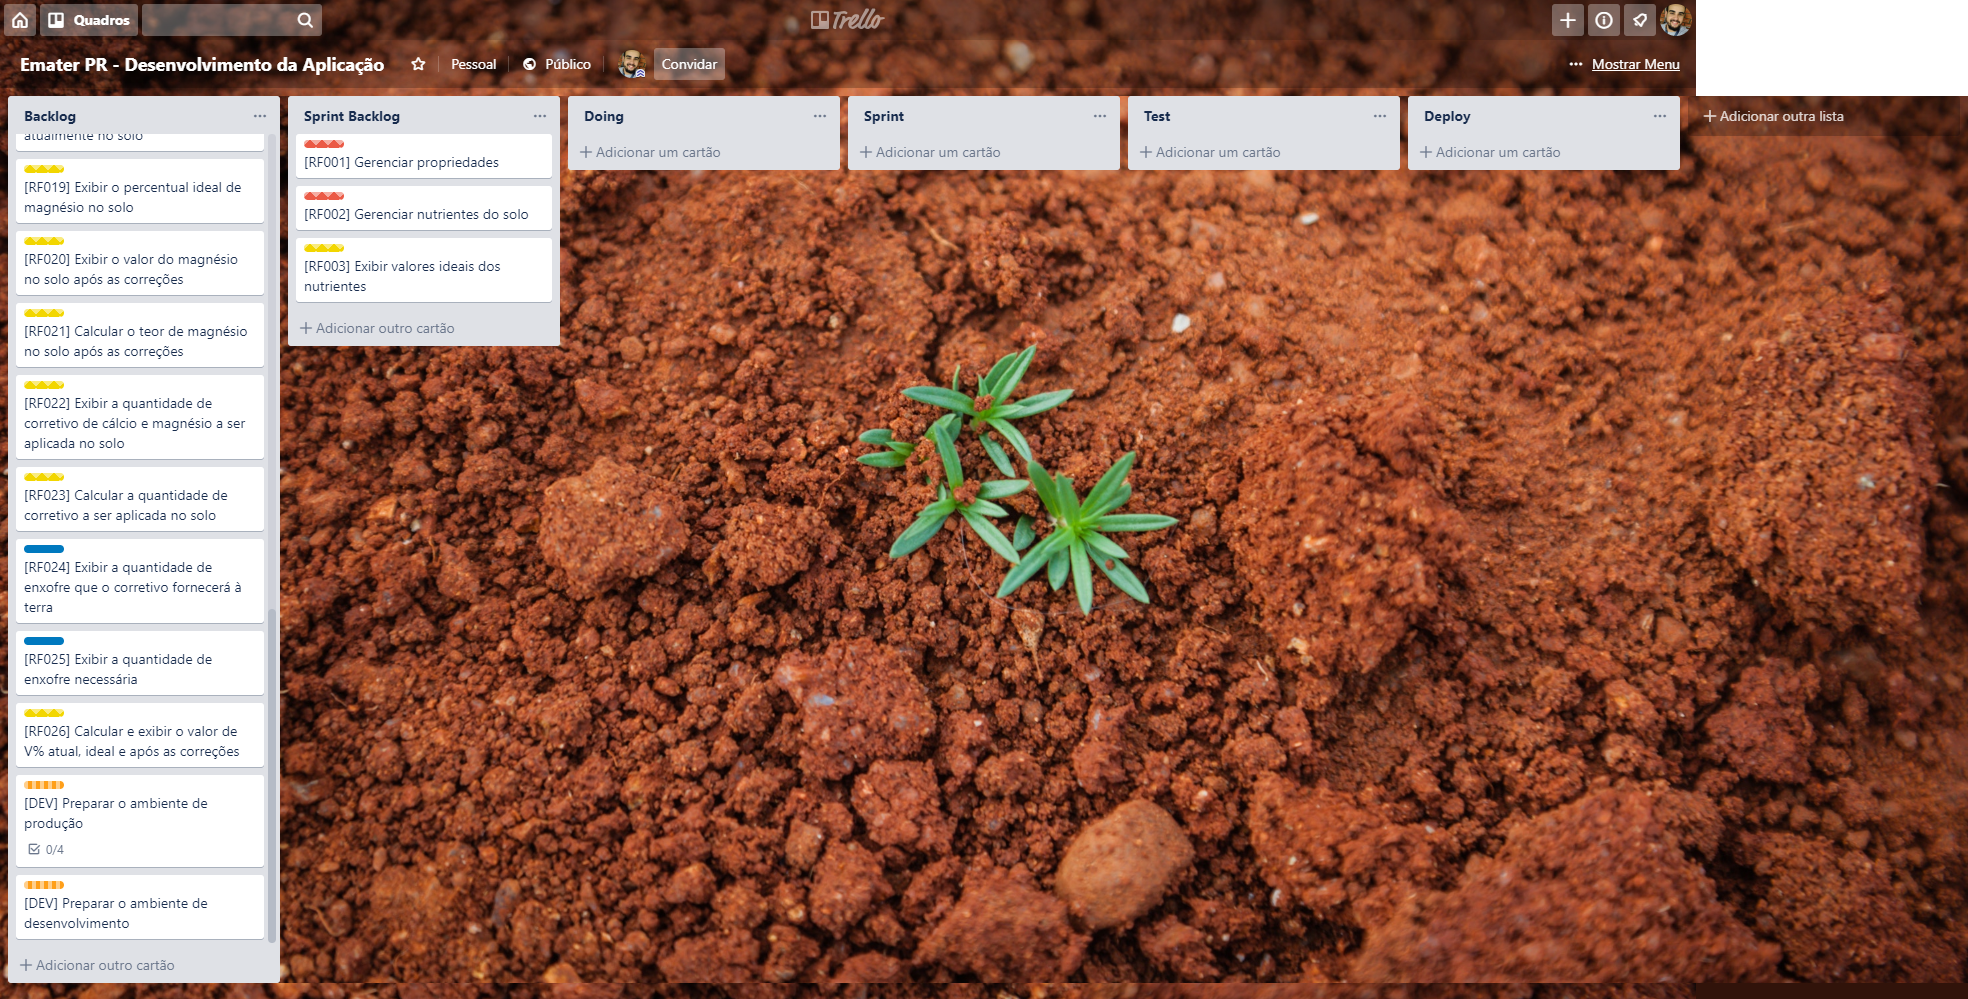
\includegraphics[width=13cm]{dados/figuras/quadro_trello.png}
    \label{fig:trelloquadro}
    \fonte{Autoria própria}
\end{figure}

\subsection{Test Driven Development}
\label{subsec:tdd}

Para aumentar a confiabilidade e a qualidade, um sistema requer a presença de testes automatizados \cite{myers2004art}. Devido a esse fato, o sistema será desenvolvidos seguindo os princípios do \textit{Test} \textit{Driven} \textit{Development} (TDD). Esta técnica tem como principal característica a escrita do teste antes da implementação da funcionalidade, sendo assim, há uma inversão de lógica quando comparamos aos modelos tradicionais \cite{erdogmus2005effectiveness}. A geração de testes antes da implementação da funcionalidade auxilia no desenvolvimento de sistemas mais bem estruturados, com menos problemas e mais flexíveis \cite{melnik2007empirical}.

Neste ciclo, cada iteração possui três momentos. O primeiro é o \textit{red}, no qual o teste é escrito e, como a funcionalidade ainda não está implementada, o teste deve falhar. O próximo passo é o \textit{green}, no qual a funcionalidade é escrita sem se preocupar com os conceitos de \textit{clean} \textit{code}, tendo como único objetivo passar no teste. Após passar pelo teste, o código implementado deve ser refatorado (\textit{refactor}), procurando se adequar aos padrões de código para garantir a legibilidade e a correta organização desse trecho.

Este técnica, segundo \citeonline{aniche2014test}, pode ser vantajosa para seus praticantes. Dentre essas vantagens destacam-se:

\begin{itemize}
    \item Começando pelo teste, o programador consegue pensar somente no que o código deve fazer, e assim sendo, esquece por instantes da implementação. Isso ajuda ao programador pensar nos melhores casos de teste para o trecho em desenvolvimento.
    \item Se seguido corretamente durante todo o processo de desenvolvimento, todo o código deverá ter pelo menos um teste de unidade atestando que este funciona corretamente.
    \item Como o programador deve buscar pela solução mais simples, acabará escapando de soluções complexas, muitas vezes desnecessárias.
    \item Muitas vezes o desenvolvedor tradicional gera um acoplamento ou desconexão entre as classes devido ao pensamento somente na classe que está trabalhando em um determinado momento. Porém, quando o teste é desenvolvido antes, o desenvolvedor pensa sobre como o código que está testando deve se comportar perante os outros e com isso pode tomar decisões mais inteligentes, gerando um maior reaproveitamento de código além de nomes de classes, atributos, métodos, parâmetros e retorno com nomes mais intuitivos, trazendo uma melhor qualidade ao código. 
    \item O desenvolvedor sempre está recebendo \textit{feedbacks} sobre o estado do código que foi desenvolvido, enquanto no modelo tradicional esses \textit{feedbacks} só serão gerados após o desenvolvimento de vários trechos de código.
\end{itemize}

Em suma, o TDD potencializa a quantidade de \textit{feedback} sobre o código que está sendo gerado, fazendo o programador reconhecer os defeitos antecipadamente, diminuindo o retrabalho e os custos de manutenção e aumentando a qualidade do código. 

Na figura \autoref{fig:ciclotdd}, é exemplificado o ciclo do TDD no desenvolvimento dessa aplicação.

\begin{figure}[H]
    \centering
    \caption{Modelo de aplicação do TDD no projeto}
    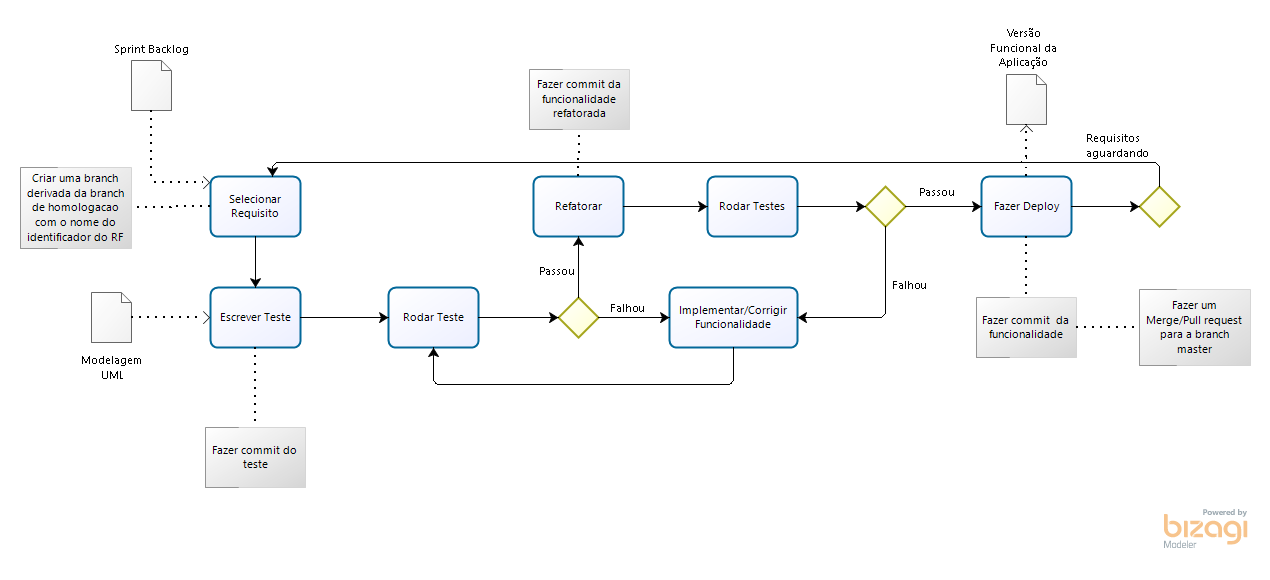
\includegraphics[width=13cm]{dados/figuras/ModeloDeAplicacaoTDD.png}
    \label{fig:ciclotdd}
    \fonte{Autoria própria}
\end{figure}

O modelo apresentado na \autoref{fig:ciclotdd} representa as etapas de uma \textit{Sprint}. É possível observar que na primeira etapa o desenvolvedor seleciona um requisito do \textit{Sprint backlog} e cria uma \textit{branch} para trabalhar nessa funcionalidade, logo após, ele deve escrever um teste, fazer um \textit{commit} então executar o teste que falhará, pois neste momento a funcionalidade ainda não foi implementada. Então, o usuário deverá seguir para a etapa de Implementação/Correção de Funcionalidade. Após concluir, deverá executar novamente o teste. Neste momento, caso o teste passe, deverá seguir para a etapa de refatoração. Após a refatoração o programador deve executar os testes de integração para ver se a nova funcionalidade se encaixou sem quebrar o sistema. Caso passe nos testes, essa funcionalidade deverá ser marcada com \textit{commit} e então enviada para \textit{deploy} no servidor de homologação para aprovação. Caso aprovado o código será incluído no servidor de produção.

O controle do estado de cada requisito será feito usando o Trello, utilizando o conceito de Kanban. Após todos os requisitos passarem pelo processo, a aplicação deve estar totalmente funcional, executando todas as tarefas que foram enumeradas na \autoref{rf:tabela}.

\section{ARQUITETURA DO SOFTWARE}
\label{sub:arquitetura}

O presente projeto seguirá o padrão arquitetural Model-View-Controller (MVC), este que \citeonline{da2012revisao} sugere uma arquitetura de software dividida em componentes, de tal forma que o código fique mais limpo e organizado, o que favorece o reaproveitamento de código e fornece uma manutenção mais segura. Porém, para que haja a independência entre os componentes, deve haver uma organização do sistema em camadas, garantindo a facilidade de escala, reuso e eficiência.

A camada \textit{model} é responsável por tratar a manipulação e persistência de dados internos, comunicando, sobretudo, com o armazenamento de dados.

Já a camada \textit{controller} é responsável pelo intermédio entre as ações que o usuário executa na interface (\textit{View}) e a resposta do servidor para essa ação, que normalmente é entregue por \textit{model}. 

Finalmente, a camada \textit{view} representa a interface pela qual o usuário interage com a aplicação. Ela define o formato de renderização mais adequado para a resposta de uma requisição.

\section{CRONOGRAMA DO PROJETO}
\label{sec:cronograma}

O gráfico abaixo representa o cronograma do projeto. O desenvolvimento será divido em sprints, que serão 

O gráfico do abaixo demonstra a distribuição das atividades do projeto em relação ao tempo. A data da primeira reunião com o professor orientador foi considerada a data inicial do cronograma, na qual foi definido o tema a ser desenvolvido. A duração de cada atividade está na unidade de dias.

\begin{landscape}

    \begin{ganttchart}
        [
            y unit title=0.4cm,
            y unit chart=0.5cm,
            vgrid,hgrid,
            title height=1,
            bar/.style={draw,fill=green},
            bar incomplete/.append style={fill=yellow!50},
            bar height=0.7
        ]{1}{36}

        \gantttitle{Junho}{6}
        \gantttitle{Julho}{5}
        \gantttitle{Agosto}{5}
        \gantttitle{Setembro}{5}
        \gantttitle{Outubro}{5}
        \gantttitle{Novembro}{5}
        \gantttitle{Dezembro}{5} \\

        \gantttitlelist{1,...,6}{1}
        \gantttitlelist{1,...,5}{1}
        \gantttitlelist{1,...,5}{1}
        \gantttitlelist{1,...,5}{1}
        \gantttitlelist{1,...,5}{1}
        \gantttitlelist{1,...,5}{1}
        \gantttitlelist{1,...,5}{1} \\

        \gantttitlelist{1,...,36}{1} \\

        \ganttbar{Desenvolvimento da Interfaces}{2}{17} \\

        \ganttbar{Desenvolvimento da API Rest}{4}{20} \\

        \ganttbar{Correções no Documento}{5}{5}
        \ganttbar{}{10}{10}
        \ganttbar{}{15}{15}
        \ganttbar{}{20}{20}
        \ganttbar{}{24}{30}\\

        \ganttbar{Entrega do Documento}{31}{30} \\

        \ganttbar{Validação pelo técnico}{5}{4}
        \ganttbar{}{10}{9}
        \ganttbar{}{15}{14}
        \ganttbar{}{20}{19} \\

        \ganttbar{Entrega parcial}{7}{6}
        \ganttbar{}{12}{11}
        \ganttbar{}{17}{16}
        \ganttbar{}{22}{21} \\

        \ganttbar{Implantação}{22}{24} \\

        \ganttbar{Testes exploratórios pelo cliente}{25}{29} \\
        \ganttbar{Correção de bugs}{25}{29} \\

    \end{ganttchart}

\end{landscape}
